\section{Brownian Motion}
\label{sec:chapter1}

\subsection{The Brownian motion discovery}



In 1827 the Scottish botanist Robert Brown published an article \cite{robert_xxvii_1828} on his observation on the pollen of \textit{Clarkia pulchella} with a lot of details on his reflection processes. His experiments were made to understand the flower reproduction, but, as he was looking through the microscope he observed some minute particles ejected from the pollen grains. At first, he thought the goal of this agitation was to test the presence of a male organ. To test this theory, he extended his observations to Mosses and \textit{Equiseta}, which were drying for a hundred years. However, the fact that this peculiar motion was still observable made him invalidate his theory. Interestingly, each time that he encountered a material that he could reduce to a fine enough powder to be suspended in water, he observed the same type of motion, although, he never understood its particle's movement.

The difficulty at this time to observe and capture such a movement made the study of what we call contemporarily Brownian motion difficult and the first theoretical work was done by Louis Bachelier in his PhD thesis ``The theory of speculation," where he described a stochastic analysis of the stock and option market. Nowadays, the mathematical description of random movement is still used in the modern financial industry. 

It is finally in 1905 that Albert Einstein theoretically state that ``bodies of microscopically visible size suspended in a liquid will perform movements of such a magnitude that they can be easily observed in a microscope" \cite{einstein_uber_1905}. A remark to make here is that in 1948 Einstein wrote a letter to one of his friends where he stated having deduced the Brownian motion ``from mechanics, without knowing that anyone had already observed anything of the kind" \cite{peter_brownian_nodate}.

It is in 1908 that Jean Perrin published his experimental work on Brownian motion. That way he could measure the Avogadro number and prove the kinetic theory that Einstein developed. I would also cite Chaudesaigues and Dabrowski, who helped Perrin to track the particles manually, half-minutes by half-minutes, for more than 3000 displacements (25 hours) and several particles. This impressive and daunting work is highly detailed in \textit{``Mouvement brownien et molécules"} \cite{perrin_mouvement_1910}. This is partly due to the results of this work that Perrin received the Nobel award in 1926.

\begin{figure}[h]
	\centering
	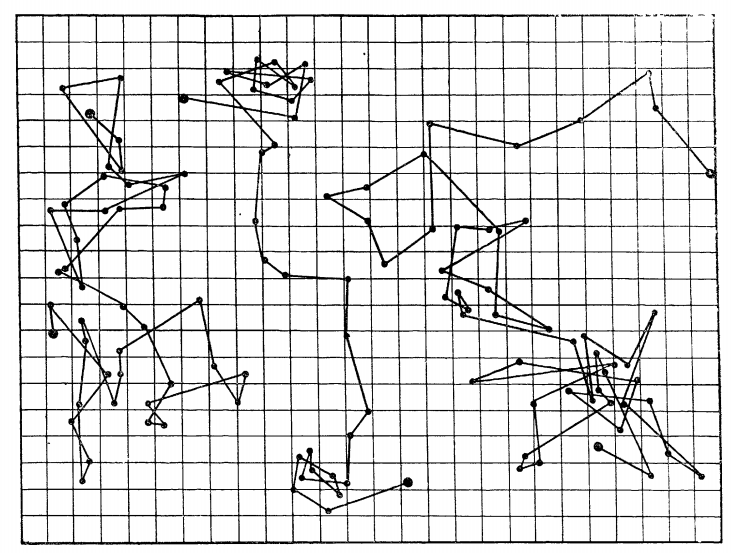
\includegraphics[scale=0.6]{02_body/chapter1/image/graph_perrin.png}
	\caption{Brownian motion of $1 ~ \mathrm{\mu m}$ particles in water tracked manually by Jean Perrin and his colleagues. The points are spaced in time by 30 seconds, and 16 divisions represent $50 ~ \mathrm{\mu m}$.}
	\label{fig:Perrin_Brownian}
\end{figure}

\subsection{Einstein's Brownian theory}

In this section we derive the main characteristics of bulk Brownian motion in the manner of Einstein in 1905 by summarizing the section 4 of \cite{einstein_uber_1905}. We then examine  the random motion of particles suspended in a liquid and its relation to diffusion, caused by thermal molecular motion. We assume that each particle motion is independent of other particles; also the motions of one particle at different times are assumed to be independent of one another provided that the time interval is not too small. Furthermore, we introduce a time interval $\tau$ which is small compared to the observation time but large enough so that  the displacements in two consecutive time intervals $\tau$ may be taken as independent events. 

For simplicity, we will here look only at the Brownian motion of $n$ particles in 1D along the $x$ axis. In a time interval $\tau$ the position of each particle will increase by a displacement $\Delta$, positive or negative. The number of particles $\textnormal{d}n$ experiencing a displacement lying between $\Delta$ and $\Delta + \textnormal{d}\Delta$ in a time interval $\tau$ is written as:

\begin{equation}
	\textnormal{d}n = n\varphi(\Delta)\textnormal{d}\Delta ~,
\end{equation}

where:

\begin{equation}
	\int_{-\infty} ^{\infty} \varphi (\Delta)\textnormal{d} \Delta = 1 ~,
	\label{Eq:ein_def_phi}
\end{equation}

and $\varphi$ is the probability distribution of displacement. We assume for now, that  $\varphi$ is a Gaussian distribution, with a variance scaling linearly with $\tau$. Additionally, since such a distribution is even, it satisfies: $\varphi (\Delta) = \varphi (-\Delta)$.

Let $f(x,t)$ be the number of particles per unit volume. From the definition of the function $\varphi(\Delta)$ we can obtain the distribution of particles found at time $ t + \tau$ from their distribution at a time $t$, through:

\begin{equation}
	f(x, t+\tau) = \int_{-\infty} ^{ +\infty} f(x-\Delta, t) \varphi (\Delta) \textnormal{d}\Delta ~.
	\label{Eq:Ein_first}
\end{equation}

Since we suppose that $\tau$ is very small with respect to  $t$, we have at first order in time:

\begin{equation}
	f(x, t+\tau) \simeq f(x,t) + \tau \frac{\partial f}{\partial t} ~.
	\label{eq:e1}
\end{equation}

Besides, we can Taylor expand $f(x+\Delta, t)$ in powers of $\Delta$ since only small values of $\Delta$ contribute. We obtain:

\begin{equation}
	f(x - \Delta, t) = f(x,t) - \Delta \frac{\partial f(x,t)}{\partial x} + \frac{\Delta ^2}{2!} \frac{\partial ^2 f(x,t)}{\partial x^2} ~.
	\label{eq:e2}
\end{equation}

Combining Eqs.\ref{eq:e1}, \ref{eq:e2} and \ref{Eq:Ein_first} we obtain:

\begin{equation}
	f + \frac{\partial f}{\partial t} \tau = f \int_{-\infty}^{+\infty} \varphi(\Delta)\textnormal{d} \Delta + \frac{\partial f}{\partial x} \int_{-\infty}^{+\infty} \Delta \varphi (\Delta)\textnormal{d} \Delta + \frac{\partial ^2 f}{\partial x^2} \int_{-\infty}^{+\infty} \frac{\Delta ^2}{2} \varphi(\Delta)\textnormal{d}\Delta ~.
	\label{Eq:ein_expended}
\end{equation}

On the right-hand side, since $\varphi(x)$ is an even function, the second term vanishes. Considering Eq.~(\ref{Eq:ein_def_phi}) and invoking the following definition:



\begin{equation}
	\frac{1}{\tau} \int_{-\infty}^{+\infty} \frac{\Delta^2}{2}\varphi(\Delta)\textnormal{d}\Delta = D ~,
\end{equation}

Eq.~(\ref{Eq:ein_expended}) finally becomes:

\begin{equation}
	\frac{\partial f}{\partial t} = D \frac{\partial ^2 f}{\partial x ^2} ~.
	\label{Eq.HeatEquation}
\end{equation}


We can here recognize a partial equation of diffusion with $D$ the diffusion coefficient. We will now initiate the same position $x=0$ for all the particles at $t=0$ as in Fig.\ref{fig:bulkbrown}. $f(x,t)\textnormal{d}x$ denotes the number of particles whose positions have increased between the times  $0$ and $t$  by a quantity lying between $x$ and $x + dx$ such that we must have:

\begin{equation}
	f(x \ne 0, t=0) = 0 \text{ and } \int_{-\infty}^{+\infty}f(x,t)dx = n ~.
\end{equation}

The solution Eq.~(\ref{Eq.HeatEquation}) is then the Green's function of the heat equation in the bulk:


\begin{equation}
f(x,t) = \frac{1}{\sqrt{4\pi D}} \frac{\exp \left(\frac{-x^2}{4Dt} \right)}{\sqrt{t}} ~.
\end{equation}

From this solution we can see that the mean value of the displacement along the $x$ axis is equal to $0$ and the square root of the arithmetic mean of the squares of displacements (that we commonly call the Root Mean Square Displacement (R\gls{MSD}))  is given by:
\begin{equation}
	\lambda _x = \sqrt{\langle \Delta ^2 \rangle} =  \sqrt{2Dt}.
	\label{Eq:MSD_ein}
\end{equation}

The mean displacement is thus proportional to the square root of time. This result is generally the first behavior that we check when we study Brownian motion. In 3D, the square root of the \gls{MSD} is given by $\lambda_x \sqrt{3}$.

Previously in his article \cite{einstein_uber_1905}, Einstein had found by writing the thermodynamic equilibrium of a suspension of particles that the diffusion coefficient of a particle should read:

\begin{equation}
	D = \frac{R T}{N_\mathrm{A}}\frac{1}{6\pi \eta a} = \frac{k_\mathrm{B}T}{6 \pi \eta a}
	~,
	\label{Eq:D_einstein}
\end{equation}

\nomenclature{$R$}{Gas constant}
\nomenclature{$N_\mathrm{A}$}{Avogrado constant}
\nomenclature{$k_\mathrm{B}$}{Boltzmann Constant}
\nomenclature{$D$}{Diffusion coefficient, see Eq.~(\ref{Eq:D_einstein})}

with $R$ the gas constant, $T$ the temperature, $N_\mathrm{A}$ the Avogadro number, $\eta$ the fluid viscosity and $k_\mathrm{B}$ the Boltzmann constant. Thus, an experimental measurement of $D$ lead to a measurement of the Avogadro number since:

\begin{equation}
	N_\mathrm{A} = \frac{t}{\lambda_x^2} \frac{RT}{3\pi \eta a} ~.
\end{equation}

Furthermore, measuring $N_\mathrm{A}$ also gives us the mass of atoms and molecules since the mass of a mole is known; as an example the mass of an oxygen atom will be given by $\left(\frac{16}{N_\mathrm{A}}\right)$ and the mass of a water molecule by $\frac{18}{N_\mathrm{A}}$. Finally, Einstein ends up is article \cite{einstein_uber_1905} by writing, \textit{``Let us hope that a researcher will soon succeed in solving the problem posed here, which is of such importance in the theory of heat!"} I would like here to emphasize the importance of solving this problem at the very beginning of the 20th century. At this time two hypotheses about the fundamental matter components existed, one involving energy and a continuum description in terms of field, and the other one, discrete atoms, especially supported by Boltzmann and his kinetic theory of gases, used by Einstein. Due to a lot of conceptual misunderstandings and experimental error scientist such as Svedberg or Henri thought that Einstein's theory was false \cite{genthon_concept_2020} by even suggesting that the statistical properties of Brownian motion were changing with the pH of the solution. It is finally in 1908 that Chaudesaigues and Perrin published all the evidence to prove Einstein's theory mainly by their ability to create particle emulsions of well-controlled radii. 

\begin{figure}[!h]
	\centering
	\includegraphics{02_body/chapter1/image/brown_exemple.pdf}
	\caption{Simulation of over-damped Brownian motion in the bulk (see Eq.~(\ref{Eq.shortnumlangevin})) of $1 ~ \mathrm{\mu m}$ particles in water. On the top each line represents the trajectory of a Brownian particle over 100 seconds. A total of 100 trajectories are shown. On the bottom, bullets represent the Mean Square Displacement (\gls{MSD}) computed from the simulated trajectories. The plain black line represents Einstein's theory, which is computed from the square of Eq.~(\ref{Eq:MSD_ein}).\href{https://github.com/eXpensia/Confined-Brownian-Motion/blob/main/02_body/chapter1/image/simple_Brownian.ipynb}{\faGithub}}
	\label{fig:bulkbrown}
\end{figure}

\subsection{The Langevin Equation}

in physics we generally describe Brownian motion through a particular Stochastic Differential Equations (\gls{SDE}). This model was introduced in 1908 by Langevin \cite{langevin_sur_1908}, this model is now used by the major part of physicists working on random processes. The Langevin equation for a free colloid reads:

\begin{equation}
	m \textnormal{d}V_t  = - \gamma V_t \textnormal{d}t + g \textnormal{d}W ~,
	\label{Eq.langevinEquation}
\end{equation}

\nomenclature{$V_t$}{Velocity of a particle}
\nomenclature{$g$}{Noise amplitude}
\nomenclature{$T$}{Temperature}

with $m$ the mass and $V_t$ the velocity of the particle. This \gls{SDE} is the Newton's second law, relating the particle momentum change on the left-hand side of the equation to forces on the right-hand side. We see that the total force applied on the particle is given by two terms: a friction term, with a Stokes-like fluid friction coefficient $\gamma$, a random force with $g$ that we will detail for a spherical particle, $\mathrm{d}B_t$ a random noise which has a Gaussian distribution of zero mean thus:

\begin{equation}
	\langle \textnormal{d}W \rangle  = 0~,
	\label{Eq.meandbt}
\end{equation}

and variance equal to: 

\begin{equation}
	\langle \textnormal{d}W ^2 \rangle = \textnormal{d}t~.
	\label{Eq.meandbt2}
\end{equation}

For a spherical particle, the friction term is given by the Stoke's formula: $\gamma = 6\pi \eta a$ with $\eta$ the fluid viscosity and $g$ the particle radius. Thus, we can derive the mean value of the particle velocity as:

\nomenclature{$\eta$}{Fluid viscosity}
\nomenclature{$\gamma$}{Friction coefficient}

\begin{equation}
	\left\langle   \textnormal{d}V_t \right\rangle = - \frac{\gamma}{m} \langle V_t \rangle \textnormal{d}t  + \frac{g}{m} \langle  \textnormal{d}W \rangle ~,
	\label{Eq.langevinsd}
\end{equation}

\nomenclature{$m$}{Mass of a particle}
with the properties of $dB_t$ given by Eq.~(\ref{Eq.meandbt}), it becomes:

\begin{equation}
	\langle  \textnormal{d}V_t \rangle = - \frac{\gamma}{m} \langle V_t \rangle \textnormal{d}t ~.
	\label{Eq.dvt}
\end{equation}

Moreover, without a loss of generality, the average of a variable $x$, $\langle x \rangle$, is done over a set of $N$ observations $\{x_i\}$ such as:

\begin{equation}
	\langle x \rangle = \frac{1}{N} \sum _{i=1}^N x_i ~,
\end{equation}

one can then show that:

\begin{equation}
	\frac{\textnormal{d}}{\textnormal{d}t}\langle x \rangle = \frac{\textnormal{d}}{ \textnormal{d}t} \left[\frac{1}{N} \sum _{i=1}^N x_i \right] = 
	\frac{1}{N} \sum _{i=1}^N \frac{\textnormal{d}}{ \textnormal{d}t} x_i = \langle\frac{\textnormal{d}}{\textnormal{d}t} x \rangle ~.
\end{equation}

The latter thus shows that it is possible to invert average value $\langle \cdot \rangle$ and a derivative. Therefore, Eq.~(\ref{Eq.dvt}) becomes:

\begin{equation}
	\frac{ \textnormal{d}}{\textnormal{d}t}\langle V_t \rangle = - \frac{\gamma}{m} \langle V_t \rangle ~,
\end{equation}

which has a familiar solution:
\begin{equation}
	\langle V_t (t) \rangle =   V_0 \mathrm{e}^{-\frac{\gamma}{m} t}~,
	\label{Eq.int_V_langevin}
\end{equation}

with $V_0$ an initial velocity. This result shows that the average of the velocity should decay to zero with a characteristic time $\tau_\mathrm{B} = \frac{m}{\gamma}$. For instance, the polystyrene particles used during my experiments which are micrometric we have $\tau_\mathrm{B} \approx 10^{-7}$ s. This signifies that if we measure the displacements of a particle with a time interval $ \tau  >> \tau _\mathrm{B} $ the displacement can be taken as independent events as it was stated by Einstein. In physical terms, this means that we are in the over-damped regime, in this case the Langevin equation reads:

\begin{equation}
-\gamma V_t \textnormal{d}t  + g  \textnormal{d}W = 0~.	
\label{Eq.overdamped_SDE}
\end{equation}

The experiments done during my thesis used a video camera that can reach a maximum of hundreds frames per second (\gls{fps}) reaching time steps of $\approx 10^{-2}$ s. Therefore, all my work falls into the over-damped regime. Before focusing definitely on Eq.~(\ref{Eq.overdamped_SDE}), we can use Eq.~(\ref{Eq.langevinsd}) to characterize further the unknown coefficient $g$. To do so we compute the mean square value of Eq.~(\ref{Eq.langevinsd}), starting by taking the second order Taylor expansion:


\begin{equation}
	\begin{aligned}
		\textnormal{d}\left(V_t^2\right) &\simeq \frac{\partial V_t ^ 2}{\partial V_t} \textnormal{d} V_t + \frac{1}{2} \frac{\partial ^2 V_t^2}{\partial V_t ^2} \left( \textnormal{d}V_t \right)^2  \\
		& = 2 V_t \textnormal{d}V_t + (\textnormal{d}V_t)^2 \\ 
	\end{aligned}
	\label{Eq.compute1}
\end{equation}

combining Eqs.~(\ref{Eq.langevinEquation})~and~(\ref{Eq.compute1}), we obtain by only keeping  the terms of order $\textnormal{d}t$:

\begin{equation}
	\textnormal{d}\left(V_t^2\right) = 2V_t\left( -\frac{\gamma}{m}V_t\textnormal{d}t + \frac{g}{m}\textnormal{d}W  \right) + \frac{g^2}{m^2}\textnormal{d}W ^2 ~. 
\end{equation}

Thus, the average value of $ \textnormal{d}(V_t ^2)$ reads:

\begin{equation}
	\langle \textnormal{d}(V_t ^2)\rangle = -2 \frac{\gamma}{m} \langle V_t ^2 \rangle \textnormal dt + 2 \frac{g}{m} \langle V_t \textnormal{d}W \rangle + \frac{g^2}{m^2} \langle \textnormal{d}W ^2 \rangle~.
	\label{Eq.dvt2}
\end{equation} 

Moreover, since $\textnormal{d}W$ is chosen independently of the velocity $V_t$, one can write $\langle V_t \textnormal{d}W \rangle $ = $\langle V_t \rangle \langle \textnormal{d}W \rangle  =0 $. Taking the latter remark into account and the fact that $\langle \textnormal{d}W ^2\rangle = \textnormal{d}t $, Eq.~(\ref{Eq.dvt2}) becomes:

\begin{equation}
	\langle d(V_t^2) \rangle = \left[-2 \frac{\gamma}{m} \langle V_t ^2 \rangle + \frac{g^2}{m^2}\right]\textnormal{d}t~.
\end{equation}

Since equilibrium averages in thermodynamics must become time independent, we have $\langle d(V_t^2) \rangle = 0$, thus:

\begin{equation}
	\langle V_t ^2\rangle = \frac{g ^2}{2 \gamma m}~. 
\end{equation}

Besides, from the equipartition of energy we also know that:

\begin{equation}
	\langle \frac{1}{2} m V_t ^2 \rangle  = \frac{1}{2} k_\mathrm{B} T~.
\end{equation}

The latter equation permits a direct determination of the amplitude of the noise $g$: 

\begin{equation}
	g = \sqrt{2k_\mathrm{B}T \gamma}~.
\end{equation}

The latter result permits computing the amplitude of the random force in the Langevin equation. Taking the over-damped Langevin equation, it reads:

\begin{equation}
	V_t\textnormal{d}t  = \sqrt{2\frac{k_\mathrm{B}T}{\gamma}} \textnormal{d}W 
	\label{Eq.v_t_ovdmp}
\end{equation}

Furthermore, one can write the position of the particle $X_t$ at a time $t$, such as:

\begin{equation}
	X_t = \int _0 ^t V_{t'}dt'~,
	\label{Eq:particle_position}
\end{equation}

where we can suppose at the initial time $t=0$ that $X_0 = 0$. Computing 
$\langle X_t^2 \rangle$ using Eqs.~(\ref{Eq.v_t_ovdmp}),~(\ref{Eq:particle_position})~and~(\ref{Eq.meandbt2}) thus gives:

\begin{equation}
	\langle X_t ^2 \rangle =  2\frac{k_\mathrm{B}T}{\gamma}t = 2Dt
	\label{Eq.xt2}
\end{equation}

By relating $\langle X_t ^2 \rangle$ to the Mean Square Displacement (\gls{MSD}) to the initial position such as:

\begin{equation}
	\textnormal{MSD} = \langle (X_0 - X_ t)^2 \rangle =  \langle X_t ^2 \rangle~,
\end{equation}


we obtain that the \gls{MSD} should be linear with the time. This result confirms that using the over-damped Langevin equation, leads to the Einstein's result Eq.~(\ref{Eq:MSD_ein}). Where one can identify the diffusion coefficient of the particle to be $D = k_\mathrm{B}T / \gamma$. Additionally, the latter identity is called the Stokes-Einstein  relation.


Additionally, the Langevin equation can be used to compute correlator such as the velocity correlator $ \langle V_{t'}V_{t''} \rangle$ that we will detail below. Indeed, if we use the full-Langevin equation, $\langle X_t ^2 \rangle$ cannot be easily computed since $m\textnormal{d} V_t$ does not vanish. We would thus need to rewrite Eq.~(\ref{Eq.xt2})  using the velocity correletor such as:

\begin{equation}
	\langle X_t ^ 2 \rangle  = \int _0 ^ {t} \int _0 ^{t} \langle V_{t'}V_{t''} \rangle dt'dt'' ~.
	\label{Eq.int_msd}
\end{equation}

Let us now study how the two-point correlator function $ \langle V_{t'}V_{t''} \rangle $, using the full-Langevin equation multiplied by $V_0$ and following the same steps as for Eq.~(\ref{Eq.int_V_langevin}), one  has:

\begin{equation}
	\langle V_t V_0 \rangle = \langle V_0 ^2 \rangle \mathrm{e}^{-t/\tau_{\mathrm{B}}}~.
\end{equation}

As the equilibrium state is invariant under temporal translation and assuming that $V_0$ has an equilibrium steady-state distribution with $\langle V_0^2 \rangle = k_\mathrm{B} T / m$ we have:

\begin{equation}
	\langle V_t V_t' \rangle = \frac{k_\mathrm{B}T}{m} \mathrm{e}^{-|t-t'|/\tau_{\mathrm{B}}}~.
\end{equation}

One can solve Eq.~(\ref{Eq.int_msd}) by splitting the integral in two parts, where $t'>t''$ and $ t' < t''$:

\begin{equation}
	\begin{aligned}
		\langle X_t ^2 \rangle & =    \frac{k_\mathrm{B}T}{m}  \int _0 ^t \textnormal{d}t' \int _0 ^{t'} \textnormal{d}t'' \mathrm{e} ^ {- |t' - t''| / \tau_\mathrm{B}} = 2 \frac{k_\mathrm{B}T}{\gamma} \left( \int_0 ^t \textnormal{d}t' \left[1 - \mathrm{e}^{-t'/\tau_\mathrm{B}} \right] \right) \\
		& = 2 \frac{k_\mathrm{B} T}{\gamma} \left( t - \tau_\mathrm{B} \left[ 1 - \mathrm{e}^{-t/\tau_\mathrm{B}} \right] \right) ~.
	\end{aligned}
\end{equation}

We can extract two results from that equation. At a short time $t << \tau_\mathrm{B}$, one has:

\begin{equation}
	\begin{aligned}
		\langle X_t ^2 \rangle & \simeq  2 \frac{k_\mathrm{B} T}{\gamma} \left( t - \tau_\mathrm{B} \left[ 1 - 1 + \frac{t}{\tau_\mathrm{B}} - \frac{t^2}{ 2 \tau_\mathrm{B} ^2}\right]         \right) \\
		& = \frac{k_\mathrm{B} T}{m} t^2 ~.
	\end{aligned}
	\label{Eq.shorttimemsd}
\end{equation}

This is the ballistic regime. If one can experimentally explore times shorter than $\tau _ \mathrm{B} $ one will then measure the instantaneous velocity of the particle. At longer times, $t >> t_\mathrm{B}$, the \gls{MSD} is given by:

\begin{equation}
	\langle X_t ^2 \rangle \simeq 2 \frac{k_\mathrm{B}T}{\gamma} t = 2Dt ~.
	\label{eq:longtimemsd}
\end{equation}

This is the diffusive regime where the \gls{MSD}, as found earlier, Eq.~(\ref{Eq.xt2}) with the over-damped Langevin equation. To study this different result, it can be interesting to simulate the Brownian motion.

\subsection{Numerical simulation of bulk Brownian motion}

\subsubsection{The numerical Langevin Equation}

\begin{figure}[!hb]
	\centering
	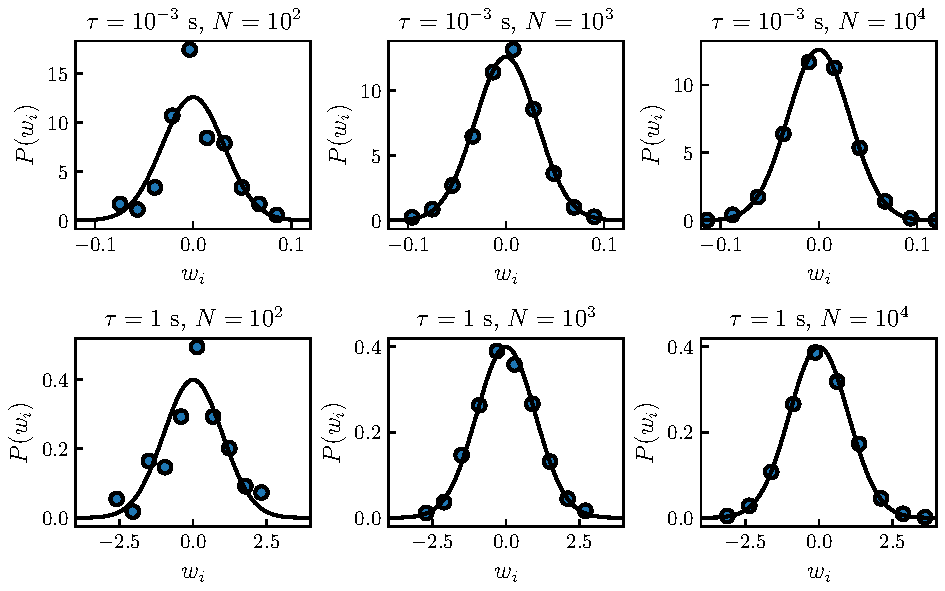
\includegraphics{02_body/chapter1/image/noise_simulation/exemple.pdf}
	\caption{Bullets represents the probability density function of $w_i$, a Gaussian-distributed number with a mean value $\langle w_i \rangle$ and a variance $\langle w_i ^2 \rangle  = \tau$. The plain black line is a Gaussian distribution of zero mean and a variance $\tau$ (see Eq.~(\ref{eq.pwi})). In the first row, the simulation is done with $\tau = 10^{-3}$ s and $\tau = 1$ s on the second one. Each column corresponds to a number $N$ of draws. From the left to the right: $N=10^2, ~10^3 \text{ and } 10^4$.\href{https://github.com/eXpensia/Confined-Brownian-Motion/blob/main/02_body/chapter1/image/noise_simulation/noise_simulation.ipynb}{\faGithub}}
	\label{fig:exempleprecisionwi}
\end{figure}


The Langevin equation is an ordinary differential equation that can easily be numerically simulated in the bulk case. We approximate the continuous position $X_t$ of a particle at a time $t$ by a discrete-time sequence $x_i$ which is the solution of the equation at a time $t_i = i  \tau$, $\tau$ being the time step of the simulation. One can then use the Euler method to numerically write $V_t$ as:

\begin{equation}
	V_t \simeq \frac{x_i - x_{i-1}}{\tau} ~,
	\label{Eq.vtnum}
\end{equation}

and $\textnormal{d}V_t / \textnormal{d}t$ as

\begin{equation}
	\begin{aligned}
		\frac{\textnormal{d}V_t}{\textnormal{d}t} &\simeq 
		\frac{
			\frac{x_i - x_{i-1}}{\tau}
			-
			\frac{x_{i-1} - x_{i-2}}{\tau}
		}
		{\tau} \\
		& =  \frac{x_i - 2x_{i - 1} + x_{i-2}}{\tau^2} ~.
	\end{aligned}
	\label{Eq.dvtnum}
\end{equation}

The only term remaining to be computed numerically is the random term $\textnormal{d}W$. One can thus replace $\textnormal{d}W / \textnormal{d}t$ by $w_i/\tau$ \footnote{The notation $w$ was choosen since in mathematical terms, a real-valued continuous-time stochastic process such as $\textnormal{d}W$ is called a Wiener process in honor of Norbert Wiener \cite{durrett_probability_2019}.} a Gaussian distributed random number generated with a mean $\langle w_i \rangle = 0$ and a variance $\langle w_i^2 \rangle  = \tau$. The Probability Density function (PDF) of the Gaussian distribution is thus given by:

\begin{equation}
	P(w_i) = \frac{1}{\sqrt{2\pi \tau}}\textnormal{e}^{- \frac{w_i^2}{2\tau}}.
	\label{eq.pwi}
\end{equation}



The random number $w_i$ can be generated with the following Python snippet.
\begin{minted}
	[
	frame=lines,
	framesep=2mm,
	baselinestretch=1.2,
	fontsize=\footnotesize,
	obeytabs=true,
	tabsize=2,
	linenos
	]
	{python}
import numpy as np
	
tau = 0.5  # time step in seconds
wi = np.random.normal(0, np.sqrt(tau))
\end{minted}


In the latter, \mintinline{python}{random.normal()} is a built-in Numpy module that permits the generation of Gaussian-distributed random numbers.
Finally, by combining Eqs.~(\ref{Eq.vtnum})~and~(\ref{Eq.dvtnum}), the full-Langevin equation becomes:




\begin{equation}
	m \frac{x_i  - 2x_{i-1} + x_{i-2}}{\tau^2} = -\gamma \frac{x_i - x_{i-1}}{\tau} + \sqrt{2k_\mathrm{B}T\gamma} \frac{w_i}{\tau}  ~.
\end{equation}

From the latter, one can write $x_i$ as:

\begin{equation} 
	x_i = \frac{2 + \tau /\tau_\mathrm{B}}{1 + \tau / \tau_\mathrm{B} } x_{i-1} 
	- \frac{1}{1 + \tau / \tau_\mathrm{B}}x_{i-2}
	+ \frac{\sqrt{2k_\mathrm{B}T\gamma}}{m(1 + \tau/\tau_\mathrm{B})} \tau w_i ~,
	\label{Eq.numfulllangevin}
\end{equation}

where we can observe that two initial conditions are needed, \textit{i.e} the first two positions of the particle. Numerically, these positions could be randomly generated or  set to $0$. If enough statics are generated, it will not affect the results.

\subsubsection{Simulating Brownian Motion Using Python}

\begin{figure}[h]
	\centering
	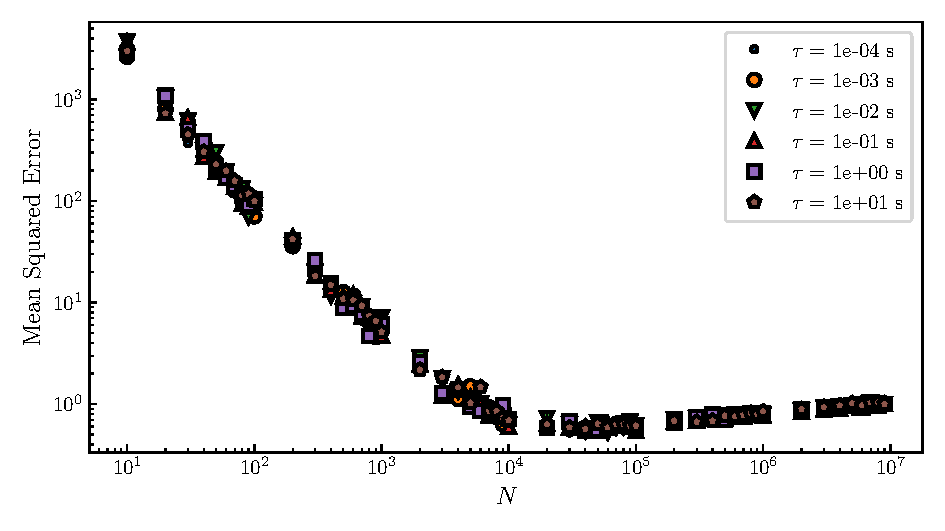
\includegraphics{02_body/chapter1/image/noise_simulation/MSE.pdf}
	\caption{Mean Relative Squared Error (\gls{MRSE}) of the Probability Density Function \gls{PDF} measured from a generation of $N$ Gaussian random numbers $w_i$ and the actual Gaussian (see Eq.~(\ref{eq.pwi})) from which the generation is done. The generation is done over a Gaussian which has a mean value $\langle w_i \rangle =0$ and variance $\langle w_i^2 \rangle = \tau$. We explore parameter ranges from $N = 10$ to $10^7$ and $\tau = 10^{-2}$ to $10$ s. \href{https://github.com/eXpensia/Confined-Brownian-Motion/blob/main/02_body/chapter1/image/noise_simulation/noise_simulation.ipynb}{\faGithub}}  
	\label{fig:MSEwi}
\end{figure}

Before, diving into the simulation, it could be interesting to wonder how long the simulation should be. Indeed, at equilibrium, for the different observables' mean values to remain constant, we should wait a sufficient amount of time. It is possible to follow a qualitative approach by generating $N$ numbers $w_i$, measuring the resulting \gls{PDF} $P_\mathrm{c}(w_i)$ and looking for how much we need to increase $N$ to have $P_\mathrm{c}(w_i) \approx P(w_i)$, under some given small-error criterion. As we can see in Fig.\ref{fig:exempleprecisionwi}, for simulations made with $\tau = 10^{-3}$ s and $\tau = 1$ s, we observe that as we increase $N$, the measured PDF, gets closer to the real one given by Eq.~(\ref{eq.pwi}). 




To have a more quantitative approach, one can compute the Mean Relative Squared Error (\gls{MRSE})) between the measured \gls{PDF} $P_\mathrm{c}(w_i)$ and the nominal function $P(w_i)$ as a function of the number $N$ of generated numbers, as:

\begin{equation}
	\textnormal{MRSE} = \left. \left\langle \frac{\left( P_\mathrm{c}(w_i) -P(w_i) \right)^2  } {P(w_i) ^2}\right\rangle \right|_N
\end{equation}

where the notation $\left. \right|_N$ denotes the average over $N$ realizations. Additionally, since we measure $P_c(w_i)$ by doing a histogram, the question of how many bins are used should be answered. It is possible to use the optimal Freedan-Diaconis rule \cite{freedman_histogram_1981} to compute the width of the bins to be used in a histogram. This rule reads:

\begin{equation}
	\textnormal{Bin width} = 2 \frac{\textnormal{IQR}(\{w_i\})}{\sqrt[3]{N}},
\end{equation}


where IQR is the interquartile range, and $\{w_i\}$ a sample of $N$ random numbers $w_i$. Moreover, one should at least take $2$ bins as a minimum. The optimal number of bins can be computed using the following Python snippet.


\begin{minted}
	[
	frame=lines,
	framesep=2mm,
	baselinestretch=1.2,
	fontsize=\footnotesize,
	obeytabs=true,
	tabsize=2,
	linenos
	]
	{python}
	
import numpy as np
	
def _iqr(wi):
	"""Function to compute interquartile range."""
		return np.subtract(*np.percentile(wi, [75, 25]))
	
	def optimal_bins(wi):
		"""
		Function to compute the optinal number of bins using Freedan-Diaconis rule.
		Input: list of random numbers | Output: optimal bins number
		"""
	
		n = int(diff(wi) / (2 * _iqr(wi) * np.power(len(wi), -1 / 3)))
	
		if n <= 2:
			return 2
		else:
			return n
\end{minted}





As we can see in Fig.\ref{fig:MSEwi}, for $\tau$ varying between $10^{-2}$ and $10$ seconds, and $N$ between $10$ and $10^6$, the \gls{MRSE} decreases as $N$ increases. Moreover, it is interesting to observe that the \gls{MRSE} is greater as $\tau$ increases for a fixed $N$ value. As an example, we would need to only generate $N = 10^{-3}$ numbers to obtain an \gls{MRSE} of $10^{-4}$ for $\tau = 0.1~\textnormal{s}$, while we would need  $N= 10^6$ for $\tau = 1 ~ \mathrm{s}$. 






Now that the Langevin equation has been numerically implemented, one could use it to simulate Brownian trajectories. A simple way to do the simulation using Python is provided in appendix.\ref{app:simfulllangevin}. A set of trajectories simulated for a fictive particle of radius $a = 1 ~ \mathrm{\mu m}$ and mass $m = 10 ~ \mathrm{\mu g}$ in water is shown in Fig.\ref{fig:inertial_langevin}-a). For such a particle, the diffusive characteristic time is $\tau_\mathrm{B} = 0.53$~s. Moreover, as one can see in Fig.\ref{fig:inertial_langevin}-b), the MSD is correctly modeled by Eq.~(\ref{Eq.shorttimemsd}) for $\tau << \tau_\mathrm{B}$, and by Eq.~(\ref{eq:longtimemsd}) for $\tau >> \tau_\mathrm{B}$. Note that for non-continuous data such as the simulation data presented here or sampled experimental trajectories, and for a given time increment $\Delta t$, the \gls{MSD} is generally defined by:

\begin{equation}
	\left\langle \Delta x^2 \right\rangle_t =  \left\langle ( x_i(t + \Delta t) - x_i(t)) ^2 \right\rangle _t ~,
	\label{Eq.msdn}
\end{equation}

where the average $ \left. \langle \rangle \right|_t $ is performed over time $t$.The following Python function can be used to numerically compute the MSD Eq.~(\ref{Eq.msdn}).

\begin{minted}
	[
	frame=lines,
	framesep=2mm,
	baselinestretch=1.2,
	fontsize=\footnotesize,
	obeytabs=true,
	tabsize=2,
	linenos
	]
	{python}
def msd(x, Dt):
	"""Function that returns the MSD for a list of time indices Dt for a trajectory x"""
	_msd = lambda x, Dt: np.mean((x[:-Dt] - x[Dt:]) ** 2)
	return [_msd(x, i) for i in t]
\end{minted}

\begin{figure}[h]
	\centering
	\includegraphics{02_body/chapter1/image/simulation_full_langevin/intertial_langevin.pdf}
	\caption{a) Set of $100$ trajectories simulated using the full-Langevin equation (see Eq.~(\ref{Eq.numfulllangevin})) for particles of a radius  $a = 1 ~\mathrm{\mu m}$ and mass $m = 10 ~\mathrm{\mu g}$ in water, with viscosity $\eta = 0.001 ~\mathrm{Pa.s}$. The simulations are done with a time step $\tau = 0.01~ \mathrm{s}$. b) Bullets represent the measured Mean Squared Displacements (\gls{MSD}) of the simulated trajectories. The plain black line represents the characteristic inertial timescale, $\tau_\mathrm{B} = m / \gamma = 0.53 ~\mathrm{s}$. The dotted line represents the \gls{MSD} in the ballistic regime (see Eq.~(\ref{Eq.shorttimemsd})), when $\Delta t \ll \tau _\mathrm{B}$. The dashed line represents the \gls{MSD} in the diffusive regime (see Eq.~(\ref{eq:longtimemsd})), when $\Delta t \gg \tau _\mathrm{B}$, $\mathrm{MSD} = 2D\Delta t$. A detailed explanation of the simulation process can be found in appendix ~\ref{app:simfulllangevin}.\href{https://github.com/eXpensia/Confined-Brownian-Motion/blob/main/02_body/chapter1/image/simulation_full_langevin/inertial_Brownian_motion.ipynb}{\faGithub}}
	\label{fig:inertial_langevin}
\end{figure}

Additionally, as we have seen earlier, the Langevin Equation can be simplified to it is over-damped version of Eq.~(\ref{Eq.overdamped_SDE}). In this case, the time step $\tau$ of the simulation should be greater than the characteristic time $\tau_\mathrm{B}$. Thus, if one is interested in the long-time statistical properties of Brownian motion one can use the over-damped Langevin equation. In this case, by putting $m=0$ into Eq.
~(\ref{Eq.numfulllangevin}), one can write $x_i$ as:

\begin{equation}
	x_i = x_{i-1} + \sqrt{2D}w_i~.
	\label{Eq.shortnumlangevin}
\end{equation}

The statistical properties at a long time could be retrieved by simulating Brownian motion using the full-Langevin equation. But, since the integration scheme used for Eq.~(\ref{Eq.numfulllangevin}) requires  $\tau \ll \tau_\mathrm{B}$, long simulation runs are necessary to retrieve the over-damped properties. A simulation of the over-damped Brownian motion trajectories using Eq.~(\ref{Eq.shortnumlangevin}) is shown in Fig.\ref{fig:bulkbrown} and is realized using the following Python Snippet.

\begin{minted}
	[
	frame=lines,
	framesep=2mm,
	baselinestretch=1.2,
	fontsize=\footnotesize,
	obeytabs=true,
	tabsize=2,
	linenos
	]
	{python}
import numpy as np
	
N = 1000  # trajectory length
D = 1  # diffusion coefficient
tau = 0.5  # time step
trajectory = np.cumsum(np.sqrt(2 * D) * np.random.normal(0, np.sqrt(tau), N))
\end{minted}

\subsubsection{Speedup using Cython}

I would like to point out that the optimization of a simple simulation of a Brownian trajectory can be interesting. Indeed, using a pure Python code as presented in the first part of appendix. \ref{app:simfulllangevin}, the simulation of one trajectory of $10^6$ steps, needs $6$ s to be computed. Thus, more than $10$ minutes are required to compute the 100 trajectories shown in Fig.~\ref{fig:inertial_langevin}. This is long and due to how Python systematically verifies what is allowed. Indeed, it verifies at each step of the \mintinline{python}{for} loop the object type of each variable and if the mathematical operation are possible. This is  generally the main drawback \cite{ampomah_qualitative_2017} of interpreted language, and the only solution is to use a compiled language (\textit{e.g} C or Fortran).

The difference between an interpreted (\textit{e.g.} Python) and compiled language (\textit{e.g.} C) lies in the result of the process of interpreting or compiling. A compiler (\textit{e.g.} gcc for the C language \href{https://github.com/gcc-mirror/gcc}{\faGithub}) translate the source code into the computer native language, and create an executable file. The execution of compiled language does not require any more translations, and hence run significantly faster. Contrariwise, an interpreted language is not translated in advance, but is done at the execution, line by line, and each time the program is executed. This process is done by the interpreter, such as Python, Matlab or Perl for their eponymous language. At each execution, the time taken by the interpreter to read and execute each line slows the process, causing execution to take more time.

To overcome this problem with Python, the \mintinline{python}{cython} package has been developed to translate in C and compile the part of the code that is long to execute, especially the \mintinline{python}{for} loops. Thus, one can transform Python source code into a hybrid Python-C code. As presented in appendix.\ref{app:simfulllangevin}, compiling the \mintinline{python}{for} loop using \mintinline{python}{cython} in the full-Langevin simulations reduces the time to generate a $10^6$-step trajectory from $6$ s to $30$ ms thus achieving a speedup  factor of $200$. Moreover, in the hybrid version, the execution time is limited by the random number generation. Indeed, it takes $ \approx 24 ~ \mathrm{ms}$ using \mintinline{python}{numpy} to generate $10^6$ $w_i$ numbers and $\approx 6$~ms for the trajectory computation. Additionally, as shown at the end of appendix.\ref{app:simfulllangevin}, even a pure C implementation of the random generation can be slower than the \mintinline{python}{numpy} one, thanks to  \mintinline{python}{numpy}'s memory optimization. Thus, by using the above mixed-language strategy, the simulation is optimal with the current tools and language at hand.

\subsection{Conclusion}

In this chapter, we have covered the history of Brownian motion, from the first observation by Robert Brown in the middle of the 19th century to its mathematical and experimental proofs in the early 20th century. We have then described mathematically the bulk Brownian motion and its important statistical properties. Finally, we have used the latter description to simulate Brownian motion using both the full-Langevin equation, and its over-damped version. 
